\chapter{Work Harder On Yourself Not On Your Job}

This lecture survives for us without validated board frames, so the transcript must carry nearly all of the mathematical burden. That is not a defect here. Rohn's mathematics is not blackboard algebra but a sequence of operational implications: what happens versus what we do, circumstances versus conduct, time versus value, job-work versus self-work. The right way to read the lecture is therefore as a chain of controlled variable shifts, each one motivated before it is compressed.

\section{From Blame to Response}

Rohn begins in confession. Personal development was hard for him because it required the surrender of a whole catalog of explanations: government, relatives, company policy, unions, wage scale, economy, interest rates, prices, circumstances. The chapter should keep that opening pressure. The later formulas mean more because they come after the comfort of blame has been explicitly renounced.

The mentor's first principle then enters as a correction to that entire frame. It is not what happens that determines the major part of the future. What happens happens to all of us. The key variable is what we do about it.

\subsection{Question \& Answer}

\paragraph{Question.} What determines the major part of the future?

\paragraph{Answer.} Not bare occurrence, but response. The first real move of the lecture is to shift causality from event to action.

We can state the cleaned relation as
\begin{equation}
\text{Major part of the future} \Longleftarrow \text{what we do about what happens}.
\end{equation}

The negation matters just as much:
\begin{equation}
\text{What happens} \not\Longrightarrow \text{major part of the future}.
\end{equation}

The lecture returns to this point more than once because it is easy to assent verbally and then continue reasoning as if events were still the real explanation.

\section{Doing Something Different Under the Same Circumstances}

Once the response variable has been isolated, the lecture immediately asks what would count as actual change. Rohn's answer is practical and deliberately small: do something different over the next ninety days than over the last ninety days. Read different books. Adopt new health disciplines. Change the texture of conduct in family life. The scale is modest because the point is not drama but mechanism.

The outer field, however, is held fixed as far as possible. We cannot change the circumstances. We can change ourselves, and therefore what we do. The lecture's first update rule may be written in cleaned form as
\begin{align}
C_{1} &= C_{0},\\
A_{1} &\neq A_{0},\\
\text{Outcome}_{1} &\neq \text{Outcome}_{0},
\end{align}
where \(C\) denotes circumstances and \(A\) action. This notation is ours, not Rohn's, but it captures his logic exactly: the environment is not the first variable to move.

That is why this section is not merely motivational. It is the lecture's first controlled experiment. Same circumstances, altered conduct, altered result. The next step is to radicalize the claim and say that even what we presently possess stands in relation to the person we have become.

\section{What We Have, and How We Change It}

Rohn's next formula is stronger and harder to hear. What we have at the moment, he says, we have attracted by the person we have become. Here the lecture stops being a general encouragement and becomes an explanation of present condition.

\begin{equation}
\text{What you have now} \Longleftarrow \text{the person you've become}.
\end{equation}

He then makes the principle hurt by applying it to biography: pennies in pocket, nothing in the bank, creditors calling, promises behind. The lecture lingers here because the point is not merely to describe poverty; it is to force the doctrine through a concrete and humiliating case. That pressure produces the natural question.

\subsection{Question \& Answer}

\paragraph{Question.} How can I change all that?

\paragraph{Answer.} By changing the person who has been attracting the present condition. The lecture's correction is not first outward but inward.

This gives us the governing formula of the whole chapter:
\begin{equation}
\text{Everything changes for you} \Longleftarrow \text{You change}.
\end{equation}

Rohn immediately unfolds it into a sequence of shorter laws:
\begin{align}
\text{Change what is inside} &\Longrightarrow \text{change what is outside for you},\\
\text{Have More} &\Longleftarrow \text{Become More}.
\end{align}

The paired imperatives that follow are not detachable slogans but compressed consequences of the same rule:
\begin{align}
\text{Wish you were better} &> \text{wish it were easier},\\
\text{Wish for more skills} &> \text{wish for fewer problems}.
\end{align}

This is the end of the lecture's first half. Everything up to here is about the internal variable. The next pivot does not abandon that variable; it chooses a countable place where we can watch it operate.

\section{The Second Beginning: Money as Diagnostic}

Rohn now restarts the lecture in a pedagogical register. In helping children understand personal development, he says, he always starts with money. That does not mean money is the highest value. It means money is easy to count.

\begin{equation}
\text{Money}=\text{a first countable diagnostic of personal development}.
\end{equation}

This is an important transition to preserve. The lecture is not suddenly becoming economic in spirit. It is using economics as a measuring device for a principle already established. Once money is chosen as the first diagnostic, the next sentence becomes the key to the whole economic block: we get paid for bringing value to the marketplace.

\section{Value, Time, and the Question of More}

The economic structure is introduced in very deliberate steps. First, pay is tied to value. Second, marketplace is glossed as reality. Third, time is admitted as necessary but demoted as the true object of payment.

\begin{align}
\text{We get paid for bringing value to the marketplace},\\
\text{Marketplace}=\text{Reality}.
\end{align}

Then comes the correction:
\begin{align}
\text{Time is required to bring value to the marketplace},\\
\text{Pay} \neq \text{Time alone},\\
\text{You get paid for the value you put in the time}.
\end{align}

\subsection{Question \& Answer}

\paragraph{Question.} Do we get paid for time or for value?

\paragraph{Answer.} Time is the medium, value is the content. The lecture's point is not that time is irrelevant, but that time alone is not what is bought.

A cautious symbolic compression, useful for note-writing though not spoken in symbols, is
\begin{equation}
P \propto V \qquad (T \text{ fixed}),
\end{equation}
where \(P\) is pay, \(V\) value, and \(T\) time.

Now the lecture can ask what it calls one of the key questions of the afternoon.

\subsection{Question \& Answer}

\paragraph{Question.} Is it possible to make more money in the same time?

\paragraph{Answer.} Yes. If the same time contains more value, then the same time can return more money.

A clean worked version is
\begin{align}
T_{1} &= T_{0},\\
V_{1} &= 2V_{0},\\
P_{1} &= 2P_{0}.
\end{align}

Rohn's spoken answer is emphatic: of course. The lecture then restates the result in operational form:
\begin{equation}
\text{Earn more money in the same time} \Longleftarrow \text{Become more valuable}.
\end{equation}

The argument is now ready for its central image.

\section{The Ladder, the Marketplace, and Opportunity}

America, Rohn says, is a ladder to climb. It is not a bed. That metaphor performs a great deal of work in a small space. It turns the same-time value argument into a picture of starting point, motion, and ascent.

\begin{align}
\text{America} &= \text{a ladder to climb},\\
\text{America} &\neq \text{a bed}.
\end{align}

The starting rung is placed near \(\$4\) an hour. The argument about whether it should be five is answered by shifting the real issue: the point of a ladder is not permanent residence at the bottom rung.

\begin{figure}[h]
\centering
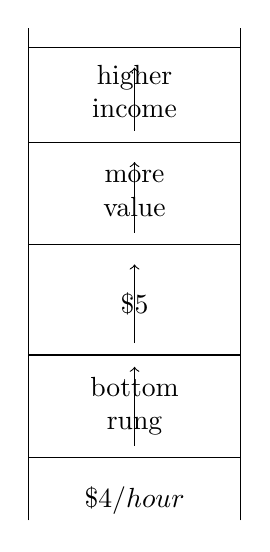
\begin{tikzpicture}
\draw (-1.35,0) -- (-1.35,6.25);
\draw (1.35,0) -- (1.35,6.25);
\draw (-1.35,0.8) -- (1.35,0.8);
\draw (-1.35,2.1) -- (1.35,2.1);
\draw (-1.35,3.5) -- (1.35,3.5);
\draw (-1.35,4.8) -- (1.35,4.8);
\draw (-1.35,6.0) -- (1.35,6.0);
\node[align=center] at (0,0.25) {\(\$4/\text{hour}\)};
\node[align=center] at (0,1.45) {bottom\\rung};
\node[align=center] at (0,2.75) {\(\$5\)};
\node[align=center] at (0,4.15) {more\\value};
\node[align=center] at (0,5.45) {higher\\income};
\draw[->] (0,0.95) -- (0,1.95);
\draw[->] (0,2.25) -- (0,3.25);
\draw[->] (0,3.65) -- (0,4.55);
\draw[->] (0,4.95) -- (0,5.75);
\end{tikzpicture}
\caption{Transcript-derived ladder reconstruction. No validated board frame survives for this lecture, so the figure is drawn from the spoken sequence itself.}
\end{figure}

The lecture then makes its most delicate distinction. One may be valuable in moral, communal, familial, or spiritual ways and still not be very valuable to the marketplace. Without that distinction the chapter would become both harsher and sloppier than the lecture itself.

The practical implications are then stated with unusual bluntness:
\begin{align}
\text{Low marketplace value} &\Longrightarrow \text{Low marketplace pay},\\
\text{Demand} &\not\Longrightarrow \text{Riches},\\
\text{Climb} &> \text{wait for a raise}.
\end{align}

\subsection{Question \& Answer}

\paragraph{Question.} How do we get more money?

\paragraph{Answer.} Not by demand and not by passive waiting, but by becoming more valuable and therefore climbing.

The phone-call anecdote now serves as proof by example. First comes the surprised thought that they called him. Then comes the corrective thought: of course they called him. Who else would they call if he could get the job done? That two-step movement should remain in the chapter, because it is the anecdotal verification of the earlier formulas.

\begin{equation}
\text{Telephone call worth millions} \Longleftarrow \text{I had become valuable}.
\end{equation}

Rohn then generalizes the anecdote once more: is it possible to become worth millions, speaking economically? Of course. That line should remain close to the phone-call story, since it is the lecture's bridge from personal example back to general rule.

\section{Work Harder on Yourself Than on Your Job}

The closing secret is as compressed as anything in the lecture:
\begin{align}
\text{Work hard on your job} &\Longrightarrow \text{Make a living},\\
\text{Work hard on yourself} &\Longrightarrow \text{Make a fortune}.
\end{align}

Rohn is careful, however, to explain why this is not a cheap attack on ordinary effort. He says that even at twenty-five he was already a hard worker. He would come early, stay late, and keep going. The problem was not the amount of work. The problem was its direction. He was working hard on the job, not on himself.

That is why the last expansion matters. Self-work means skills, graces, philosophy, attitude, personality, language, communication, and ability. Economics, he says, is the least of the values that begin to change once this process is taken up. The closing agricultural sequence makes the same point in another idiom: do not try to change the seed, the soil, the sunshine, the rain, the seasons. Let the external givens be what they are, and go to work on the inside.

The chapter therefore should not end on wage arithmetic alone. It must return to the larger claim that the same personal changes that alter pay also alter the quality of one's future.

\section{Summary}

The lecture unfolds as a sequence of variable shifts. First we surrender blame and move from what happens to what we do about it. Then we move from conduct to the person we have become, and from there to the inside/outside formulas of self-change. Only after that does the lecture choose money as a countable arena, distinguish value from time, and ask whether greater value can produce greater money in the same time. The answer opens into the ladder image, the distinction between marketplace value and human worth, the rejection of demand and waiting, and the proof that value attracts opportunity. The close then gathers everything back into the larger labor of self-development.

The shortest faithful summary is still the strongest one:
\begin{equation}
\text{Everything changes for you} \Longleftarrow \text{You change}.
\end{equation}

And its most practical economic companion is this:
\begin{equation}
\text{Work on yourself} \Longrightarrow \text{Become more valuable to the marketplace}.
\end{equation}

That is the full circle of the lecture: change response, change self, change value, change result.